% ------------------------------------------------------------------------------
% TYPO3 CMS 7.3 - What's New (English Version)
%
% @author	Michael Schams <schams.net>
% @license	Creative Commons BY-NC-SA 3.0
% @link		http://typo3.org/download/release-notes/whats-new/
% @language	English
% ------------------------------------------------------------------------------
% LTXE-CHAPTER-UID:		cc6b358d-f0ed36d3-f7a72fa2-af63ccfc
% LTXE-CHAPTER-NAME:	Backend User Interface
% ------------------------------------------------------------------------------

\section{Interfaccia utente Backend}
\begin{frame}[fragile]
	\frametitle{Interfaccia utente Backend}

	\begin{center}\huge{Capitolo 1:}\end{center}
	\begin{center}\huge{\color{typo3darkgrey}\textbf{Interfaccia utente Backend}}\end{center}

\end{frame}

% ------------------------------------------------------------------------------
% LTXE-SLIDE-START
% LTXE-SLIDE-UID:		0f993826-2955e324-8b85c0c4-6073b08a
% LTXE-SLIDE-ORIGIN:	111332b8-ac46a07a-319ed582-f873bc02 English
% LTXE-SLIDE-ORIGIN:	b4dc1576-57b4854f-26a32d85-11f7c52b German
% LTXE-SLIDE-TITLE:		Feature #66173: Allow page title edit by doubleclick
% LTXE-SLIDE-REFERENCE:	Feature-66173-AllowPageTitleEditByDoubleclick.rst
% ------------------------------------------------------------------------------
\begin{frame}[fragile]
	\frametitle{Interfaccia utente Backend}
	\framesubtitle{Titolo di pagina nei moduli Pagina e Lista}

	Gli utenti possono modificare il titolo della pagina nei moduli "Pagina" e "Lista" con un doppio click nell'intestazione
	della pagina o sull'icona di editing.

	\begin{figure}
		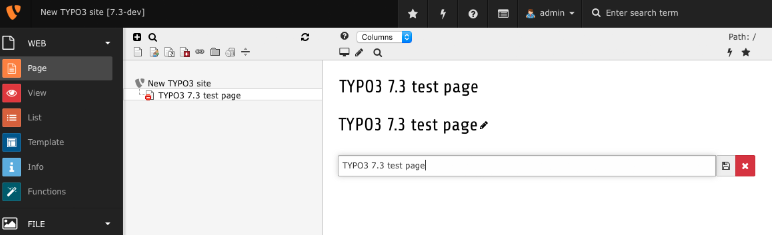
\includegraphics[width=0.9\linewidth]{BackendUserInterface/66173.png}
	\end{figure}

\end{frame}

% ------------------------------------------------------------------------------
% LTXE-SLIDE-START
% LTXE-SLIDE-UID:		af5d4b4e-6f06d3c5-a31df487-9ff512f6
% LTXE-SLIDE-ORIGIN:	c17b263e-12512d4b-13d5389f-df1ec14e English
% LTXE-SLIDE-ORIGIN:	168b1424-1ebb2552-ed5bac3e-8a9ac737 German
% LTXE-SLIDE-TITLE:		Feature #67071: Processed files cleanup tool added in Install Tool
% LTXE-SLIDE-REFERENCE:	Feature-67071-ProcessedFilesCleanupToolAddedInInstallTool.rst
% ------------------------------------------------------------------------------
\begin{frame}[fragile]
	\frametitle{Interfaccia utente Backend}
	\framesubtitle{Install Tool: Cancellazione file elaborati}

	Nella sezione "Clean up", l'Install Tool dispone di una nuova funzione per rimuovere
	i file elaborati (es. thumbnail delle immagini) del FAL.\newline
	Questo diventa utile se le impostazioni grafiche vengono cambiate o dopo un aggiornamento di
	GraphicsMagick/ImageMagick, per forzare la ricreazione di tutte le immagini.

	\begin{figure}
		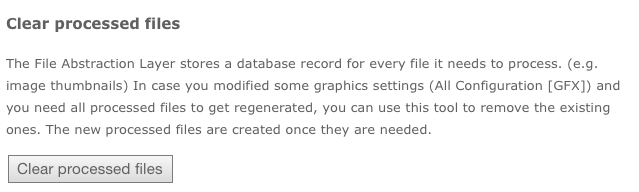
\includegraphics[width=0.6\linewidth]{BackendUserInterface/67071.png}
	\end{figure}

\end{frame}

% ------------------------------------------------------------------------------
% LTXE-SLIDE-START
% LTXE-SLIDE-UID:		07b869fd-038a29ed-50c03fb4-e8eab71a
% LTXE-SLIDE-ORIGIN:	4662a0fc-e8a91f22-2f75e0bc-800e9b63 English
% LTXE-SLIDE-ORIGIN:	daa83c1e-08d2716b-de74cbda-42361551 German
% LTXE-SLIDE-TITLE:		Feature #67319: Add field "copyright" to EXT:filemetadata
% LTXE-SLIDE-REFERENCE:	Feature-67319-AddFieldCopyrightToEXTfilemetadata.rst
% ------------------------------------------------------------------------------
\begin{frame}[fragile]
	\frametitle{Interfaccia utente Backend}
	\framesubtitle{Nuovi campi nei Meta Data del FAL}

	Il campo "\textbf{Copyright}" è stato aggiunto ai meta data del FAL
	(estensione di sistema: \texttt{filemetadata}).

	\begin{figure}
		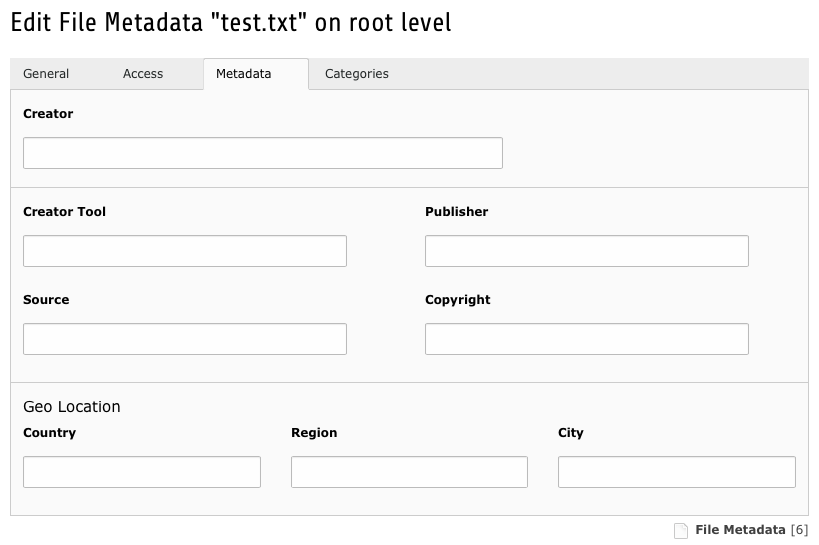
\includegraphics[width=0.6\linewidth]{BackendUserInterface/67319.png}
	\end{figure}

\end{frame}

% ------------------------------------------------------------------------------
